
\begin{enumerate}[label=\thesubsection.\arabic*.,ref=\thesubsection.\theenumi]
  \item In 
	\figref{fig:tri_med}	
	\begin{align}
	AF = BF, \,
	AE = BE, 
	\end{align}
	and the medians $BE$ and $CF$ meet at $\vec{G}$.
	Show that
\begin{align}
	ar\brak{BEC}
	=ar\brak{BFC} = \frac{1}{2}ar\brak{ABC}
	\label{eq:median-area}
\end{align}
\begin{figure}[!ht]
	\begin{center}
		{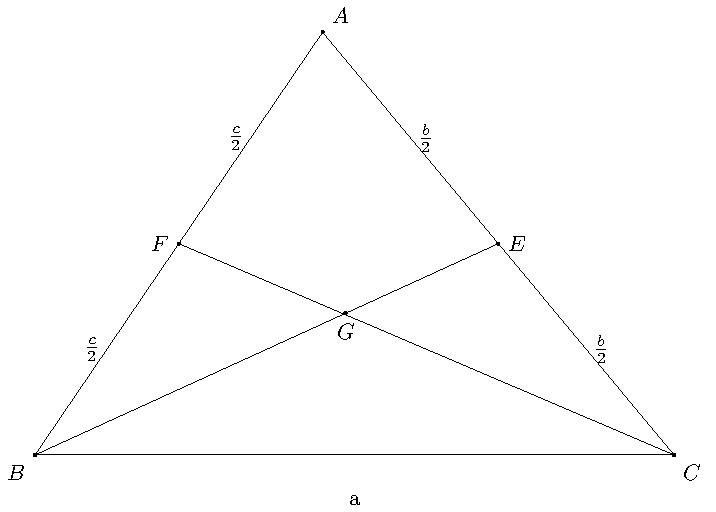
\includegraphics[width=0.6\columnwidth]{figs/trig_id/median/tri_med.pdf}}
	\end{center}
	\caption{$k_1=k_2$.}
	\label{fig:tri_med}	
\end{figure}
\solution
	From \eqref{tri:area-sin},
\begin{align}
	ar\brak{BEC} &= 
	\frac{1}{2}a\brak{\frac{b}{2}}\sin C 
	\\
	ar\brak{BFC}&=
	\frac{1}{2}a\brak{\frac{c}{2}}\sin  B
\end{align}
yielding
	\eqref{eq:median-area}.
\item The median divides a triangle into two triangle of equal area.
	\label{prob:median-area}.
\item 
	In \figref{fig:tri_med},	
	show that
\begin{align}
	ar\brak{CGE}
	=ar\brak{BGF} 
	\label{eq:median-sub-area}
\end{align}
\solution 
From 
	\figref{fig:tri_med}	
	and 
	\eqref{eq:median-area},
\begin{align}
	ar\brak{BGF}
	+
	ar\brak{BGC}
	=
	ar\brak{CGE}
	+
	ar\brak{BGC}
\end{align}
yielding 
	\eqref{eq:median-sub-area}.
\item In 
	\figref{fig:tri_med_isect},	show that
\begin{align}
	k_1=k_2
	\label{eq:med-ratio-eq}
\end{align}
\begin{figure}[!ht]
	\begin{center}
		{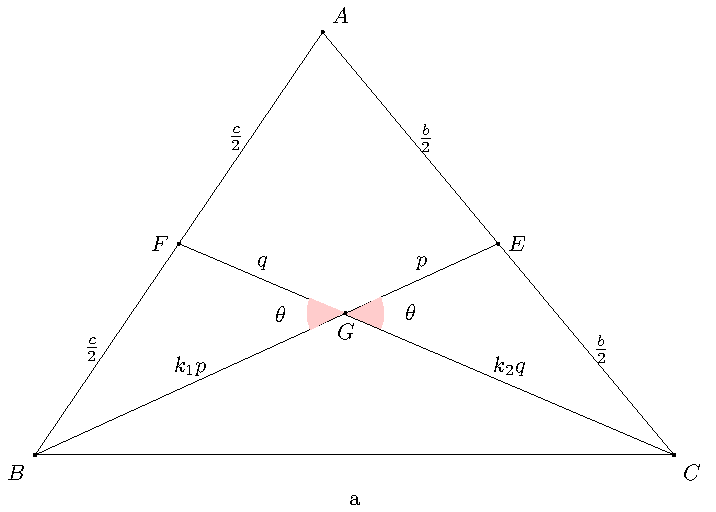
\includegraphics[width=0.6\columnwidth]{figs/trig_id/median/tri_med_isect.pdf}}
	\end{center}
	\caption{Equal areas.}
	\label{fig:tri_med_isect}	
\end{figure}
\solution
	From \eqref{eq:median-sub-area},
\begin{align}
	\frac{1}{2}p\brak{k_1q} \sin \theta
	&=\frac{1}{2}q\brak{k_2p}\sin \theta
\end{align}
	yielding \eqref{eq:med-ratio-eq}.
\item In 
	\figref{fig:tri_med_meet}, show that 	
\begin{align}
	k_3 = k
\label{eq:med-ratio-eq-k3}
\end{align}
\solution 
	From \probref{prob:median-area},
\begin{align}
\begin{split}
	ar\brak{AGE}
	&=ar\brak{CGE}
	\\
	ar\brak{AGF}
	&=ar\brak{BGF}
\end{split}
\\
\implies
\begin{split}
	\frac{1}{2}p\brak{k_3r}\sin \alpha
	&=\frac{1}{2}p\brak{kq}\sin \theta
	\\
	\frac{1}{2}q\brak{k_3r}\sin \beta
	&=\frac{1}{2}q\brak{kp} \sin \theta
\end{split}
\end{align}
yileding upon division
\begin{align}
	p\sin \alpha &= q \sin \beta
	\\
	\implies 
	\frac{1}{2}kpr\sin \alpha &= \frac{1}{2}kqr \sin \beta
	\\
	\implies ar\brak{BGD}
	&=ar\brak{CGD}
\end{align}
Thus, 
	from \probref{prob:median-area}, $AD$ is also a median.
	Consequently, 
	from
	\eqref{eq:med-ratio-eq} we obtain
\eqref{eq:med-ratio-eq-k3}.
%
\begin{figure}[H]
	\begin{center}
		{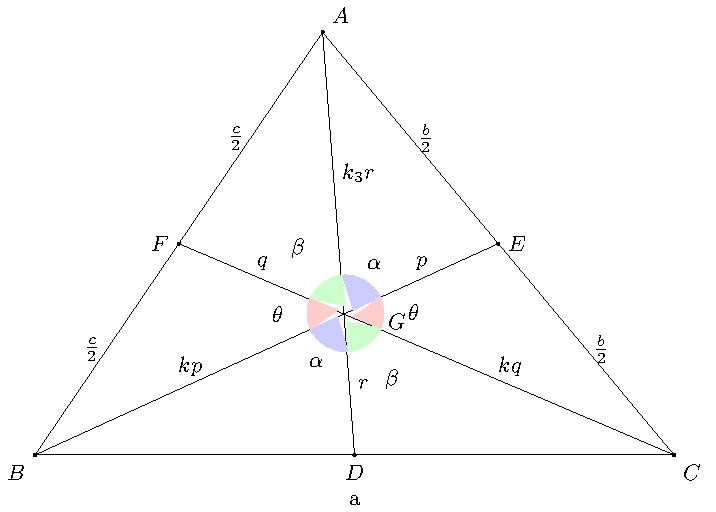
\includegraphics[width=0.6\columnwidth]{figs/trig_id/median/tri_med_meet.pdf}}
	\end{center}
	\caption{$k_3=k$.}
	\label{fig:tri_med_meet}	
\end{figure}
\item In 
	\figref{fig:tri_med_sim}, show that $k = 2$.
	\\
\solution Using the cosine formula, 
\begin{align}
	DE^2 &= \brak{\frac{b}{2}}^2+\brak{\frac{c}{2}}^2-2\brak{\frac{b}{2}}\brak{\frac{c}{2}}\cos A  
	\\
	a^2&= b^2+b^2-2bc\cos A  
	\\
	\implies DE &= \frac{a}{2}
\end{align}
$\because \triangle EGF \sim \triangle BGC, k = 2$.
\begin{figure}[H]
	\begin{center}
		{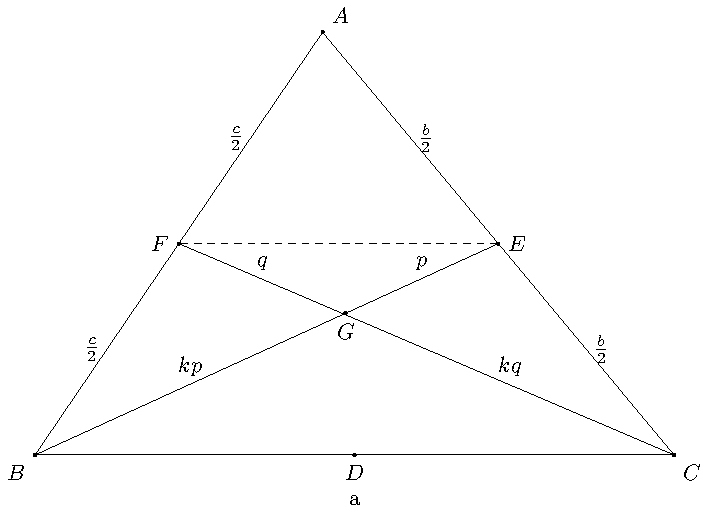
\includegraphics[width=0.6\columnwidth]{figs/trig_id/median/tri_med_sim.pdf}}
	\end{center}
	\caption{k = 2}
	\label{fig:tri_med_sim}
\end{figure}


\end{enumerate}
